\documentclass[a4paper,oneside,12pt]{article}

\NeedsTeXFormat{LaTeX2e}
\ProvidesPackage{custom}[2014/05/11 Custom Package]

\usepackage[utf8]{inputenc}
\usepackage[T1]{fontenc}
\usepackage[francais]{babel}

\usepackage[version=3]{mhchem}
\usepackage{chemfig}

\usepackage{amsmath}
\usepackage{amsthm}
\usepackage{amsfonts}

\usepackage{graphicx} 
\usepackage[top=3cm, bottom=3cm, left=3cm , right=3cm]{geometry}
%\usepackage{setspace} %doublespace, onehalfspace
\usepackage{siunitx}

\usepackage{tikz}
\usetikzlibrary{positioning}
\usetikzlibrary{shapes,arrows}

\usepackage{tabularx}
\usepackage{url} 
\usepackage{tocloft} %spacing in list of figures
\usepackage{listings} %input code
%\usepackage{multibbl} %multiplebibliography
\usepackage{hyperref}
\usepackage[babel=true]{csquotes}
\usepackage{listings}
\usepackage{color}

\usepackage{epstopdf}

\usepackage{caption}
\usepackage{subcaption}
\usepackage{float}

\newcommand{\dif}[1]{\mathrm{d}#1}
\newcommand{\e}[1]{\cdot 10^{#1}}

\endinput


\title{Tache 4 : Mini-\textsc{hazop} du noeud autour du réacteur de synthèse d'ammoniac}
\author{Groupe 1225}
\date{20 Novembre 2014}

\begin{document}

\maketitle

\section*{Question 1}

On retrouve $6$ gaz présents dans le réacteur. 
Certains ne présentent que peu de danger, 
d'autres peuvent provoquer d'importants dégats en cas de combustion.

\begin{itemize}	
	\item L'hydrogène est un gaz extrêmement inflammable et peut provoquer de grosses 
		explosions en cas de combustion. C'est le principal danger lié à sa présence. 
		En cas d'accumulation d'hydrogène dans une pièce ou un batiment, 
		sa présence peut provoquer un environnement déficient en oxygène et 
		donc provoquer la suffocation.

	\item  L'argon est présent naturellement dans l'air et n'est dangereux qu'en 
		quantités importantes. Il peut alors provoquer la suffocation.

	\item  L'azote est également naturellement présent dans l'air et n'est pas plus 
		dangereux que l'argon.

	\item  L'ammoniac est inflammable et peut donc provoquer une explosion en cas 
		d'accumulation et de combustion.

	\item  L'helium peut provoquer l'asphyxie en cas de concentration trop élevée.

	\item  Le méthane est inflammable et présente un danger d'explosion en cas 
		d'accumulation et de combustion. Il y a également un risque d'asphyxie en 
		cas d'accumulation simple.
\end{itemize}

\section*{Question 2}

Les PDF et PID se trouvent à la fin du rapport dans l'annexe \ref{ann:fluxes}.


\section*{Question 3}

\paragraph{1} Imaginons que pour une quelconque raison, il y ait une fuite de gaz inflammable, 
de l'hydrogène par exemple. Le gaz se propagerait alors dans l'atmosphère à 
une pression de $150\si{\bar}$ et à une température de $180\si{\celsius}$. 
Il s'enflammerait directement, créant ainsi une augmentation rapide de la température. 
Les canalisations, chauffées par les flammes, verraient leur pression interne augmenter 
brutalement. Les canalisations se déchireraient, entraînant la libération d'hydrogène 
supplémentaire, provoquant ainsi une déflagration.

Nous pourrions éviter le déchirement des canalisations en utilisant des disques de rupture 
au niveau de celles-ci. Si la pression interne dépasse un certain seuil, le disque de rupture 
se rompt, libérant le gaz, mais évitant la destruction des tuyauteries.

\paragraph{2} Prenons maintenant le cas où un problème survient au niveau du réacteur 
de synthèse de l'ammoniac. La réaction de synthèse

\begin{equation}
	\ce{\frac{3}{2} H2_{(g)} + \frac{1}{2} N2_{(g)} <=> NH3_{(g)}}
	\label{eq:synthesis}
\end{equation}

est une réaction exothermique ($-45.9\si{\kilo\joule}$ à $298\si{\kelvin}$). 
Elle dégage donc beaucoup de chaleur, qu'il faut traiter afin d'éviter 
une hausse trop importante de la température au sein du réacteur. 
En faisant circuler les gaz de synthèse \ce{H2 \, et \, N2},  
qui sont à $180\si{\celsius}$, dans les parois du réacteur, 
ceux-ci vont absorber une partie de la chaleur produite par la réaction. 
Nous nous apercevons donc que s'il y a une défaillance au niveau du système 
de refroidissement, par exemple si l'entrée des gaz de synthèse est bouchée, 
la température du réacteur va augmenter brusquement. Etant donné que le volume est fixe, 
la pression va augmenter proportionnellement à la température, 
jusqu'à ce qu'elle dépasse la limite supportable par les parois du réacteur. 
A ce moment-là, le réacteur explose sous l'effet de la pression.

Pour éviter cela, il faut construire le réacteur de manière à ce que 
le couvercle de celui-ci cède en premier en cas de surpression. 
Nous limitons de cette manière fortement les dommages occasionnés.

\paragraph{3} Etudions maintenant le cas d'un blackout électrique. 
L'installation est soudainement privée d'électricité. 
Les compresseurs vont donc s'arrêter, et l'apport en réactifs au niveau 
du réacteur va donc s'arrêter.
La réaction va continuer jusqu'à ce que les pressions au niveau des tuyauteries 
des réactifs et de l'ammoniac s'équilibrent.
La synthèse de l'ammoniac diminue la pression car elle réduit le nombre de moles 
de gaz présent, mais est exothermique, et puisque le refroidissement est effectué 
par les réactifs, et que le système n'est plus alimenté, le réacteur va chauffer.
Il va également falloir redémarrer le réacteur une fois l'élecricité rétablie. 
Le réacteur doit avoir le temps de refroidir afin d'éviter 
que la température ne soit trop élevée lors du redémarrage. 
Il sera cependant nécessaire de purger ou préchauffer le réacteur si
la température du réacteur est trop basse car la réaction ne se fera pas.

Nous pouvons éviter tout problème en ayant des générateurs sur site capable 
de délivrer de l'électricité en cas de blackout jusqu'à ce que 
le courant soit rétablit. 

\section*{Question 4}
% Pourquoi n’y a-t-il pas de soupape de sécurité ou de disque de rupture (les deux types 
% de dispositifs servent à protéger un équipement ou une ligne contre les surpressions) 
% sur le réacteur de synthèse du NH3 ?

Un disque de rupture est un dispositif de sécurité qui sert à protéger les installations 
contre les surpressions.
La réaction de synthèse de l'ammoniac est la réaction \ref{eq:synthesis}.
On remarque immédiatement qu'il y a une diminution du nombre de moles de gaz (d'un facteur 2) 
lorsque de l'ammoniac est produit. La loi des gazs parfait nous indique que la pression
exercée par un gaz est directement proportionnelle à son nombre de moles.
Une surpression n'est pas envisageable pour cette réaction, 
il n'y a donc pas besoin de disque de rupture sur ce réacteur.

\section*{Question 5}
% Pourquoi y a-t-il des disques de rupture sur l’échangeur 124-MC ?

L'échangeur 124-C est un dispositif permettant de transférer de la chaleur d'un fluide
vers un autre, sans que ceux-ci ne se mélangent.
On a donc un flux \emph{chaud} et un flux \emph{froid}. Le flux froid va recevoir de 
l'énergie thermique et sa température va augmenter, il faut alors prévoir des disques 
de rupture au cas où la température dépasse une certaine limite qui produirait une 
supression du gaz et pourrait endommager, voire déchirer, la paroi.
Théoriquement, le flux chaud n'a pas besoin de disque de rupture parce que le gaz qu'il 
transporte ne peut que diminuer de volume. Cependant, on peut toujours considérer le cas
d'un apport soudain et imprévu de chaleur comme une explosion extérieure, qui produirait
une augmentation de température et par conséquent de pression. 
Il devient alors nécessaire d'avoir des disques de rupture dans les deux sens de l'échangeur.


\appendix
\section{Circulation des flux de matières - PDF et PIDs}
\label{ann:fluxes}

\begin{center}
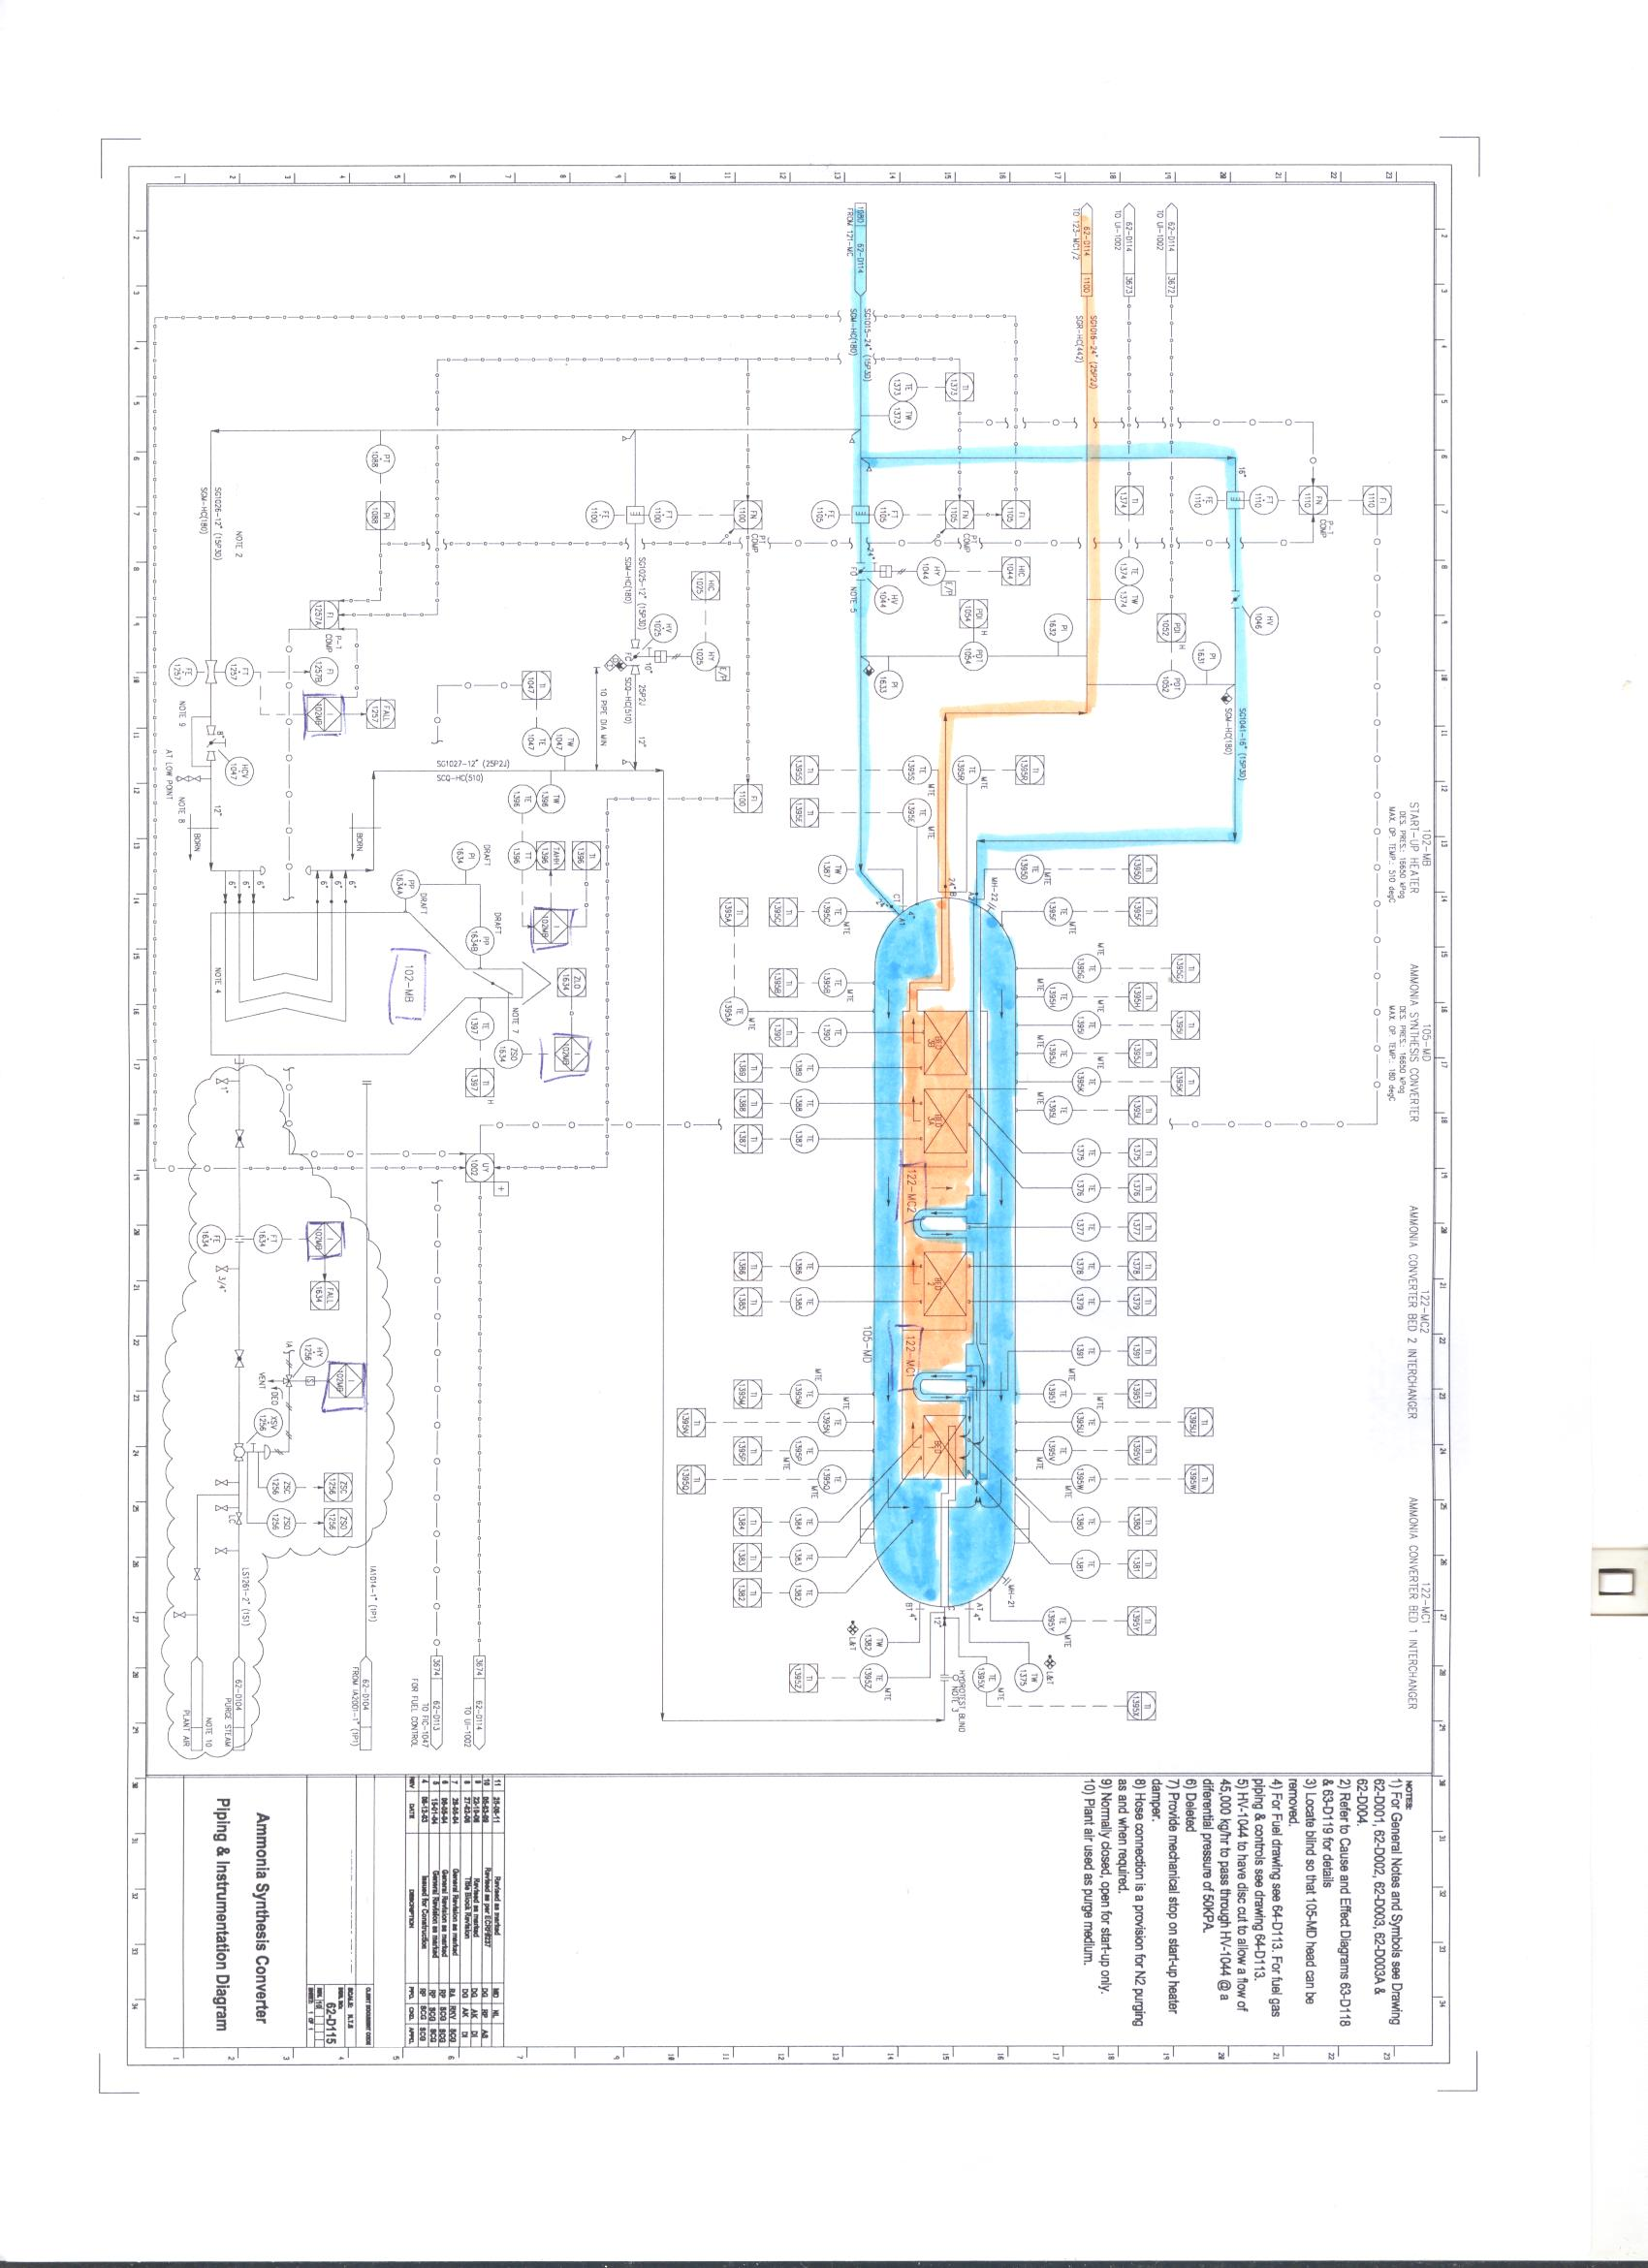
\includegraphics[scale=0.7]{img/scan1.jpg}

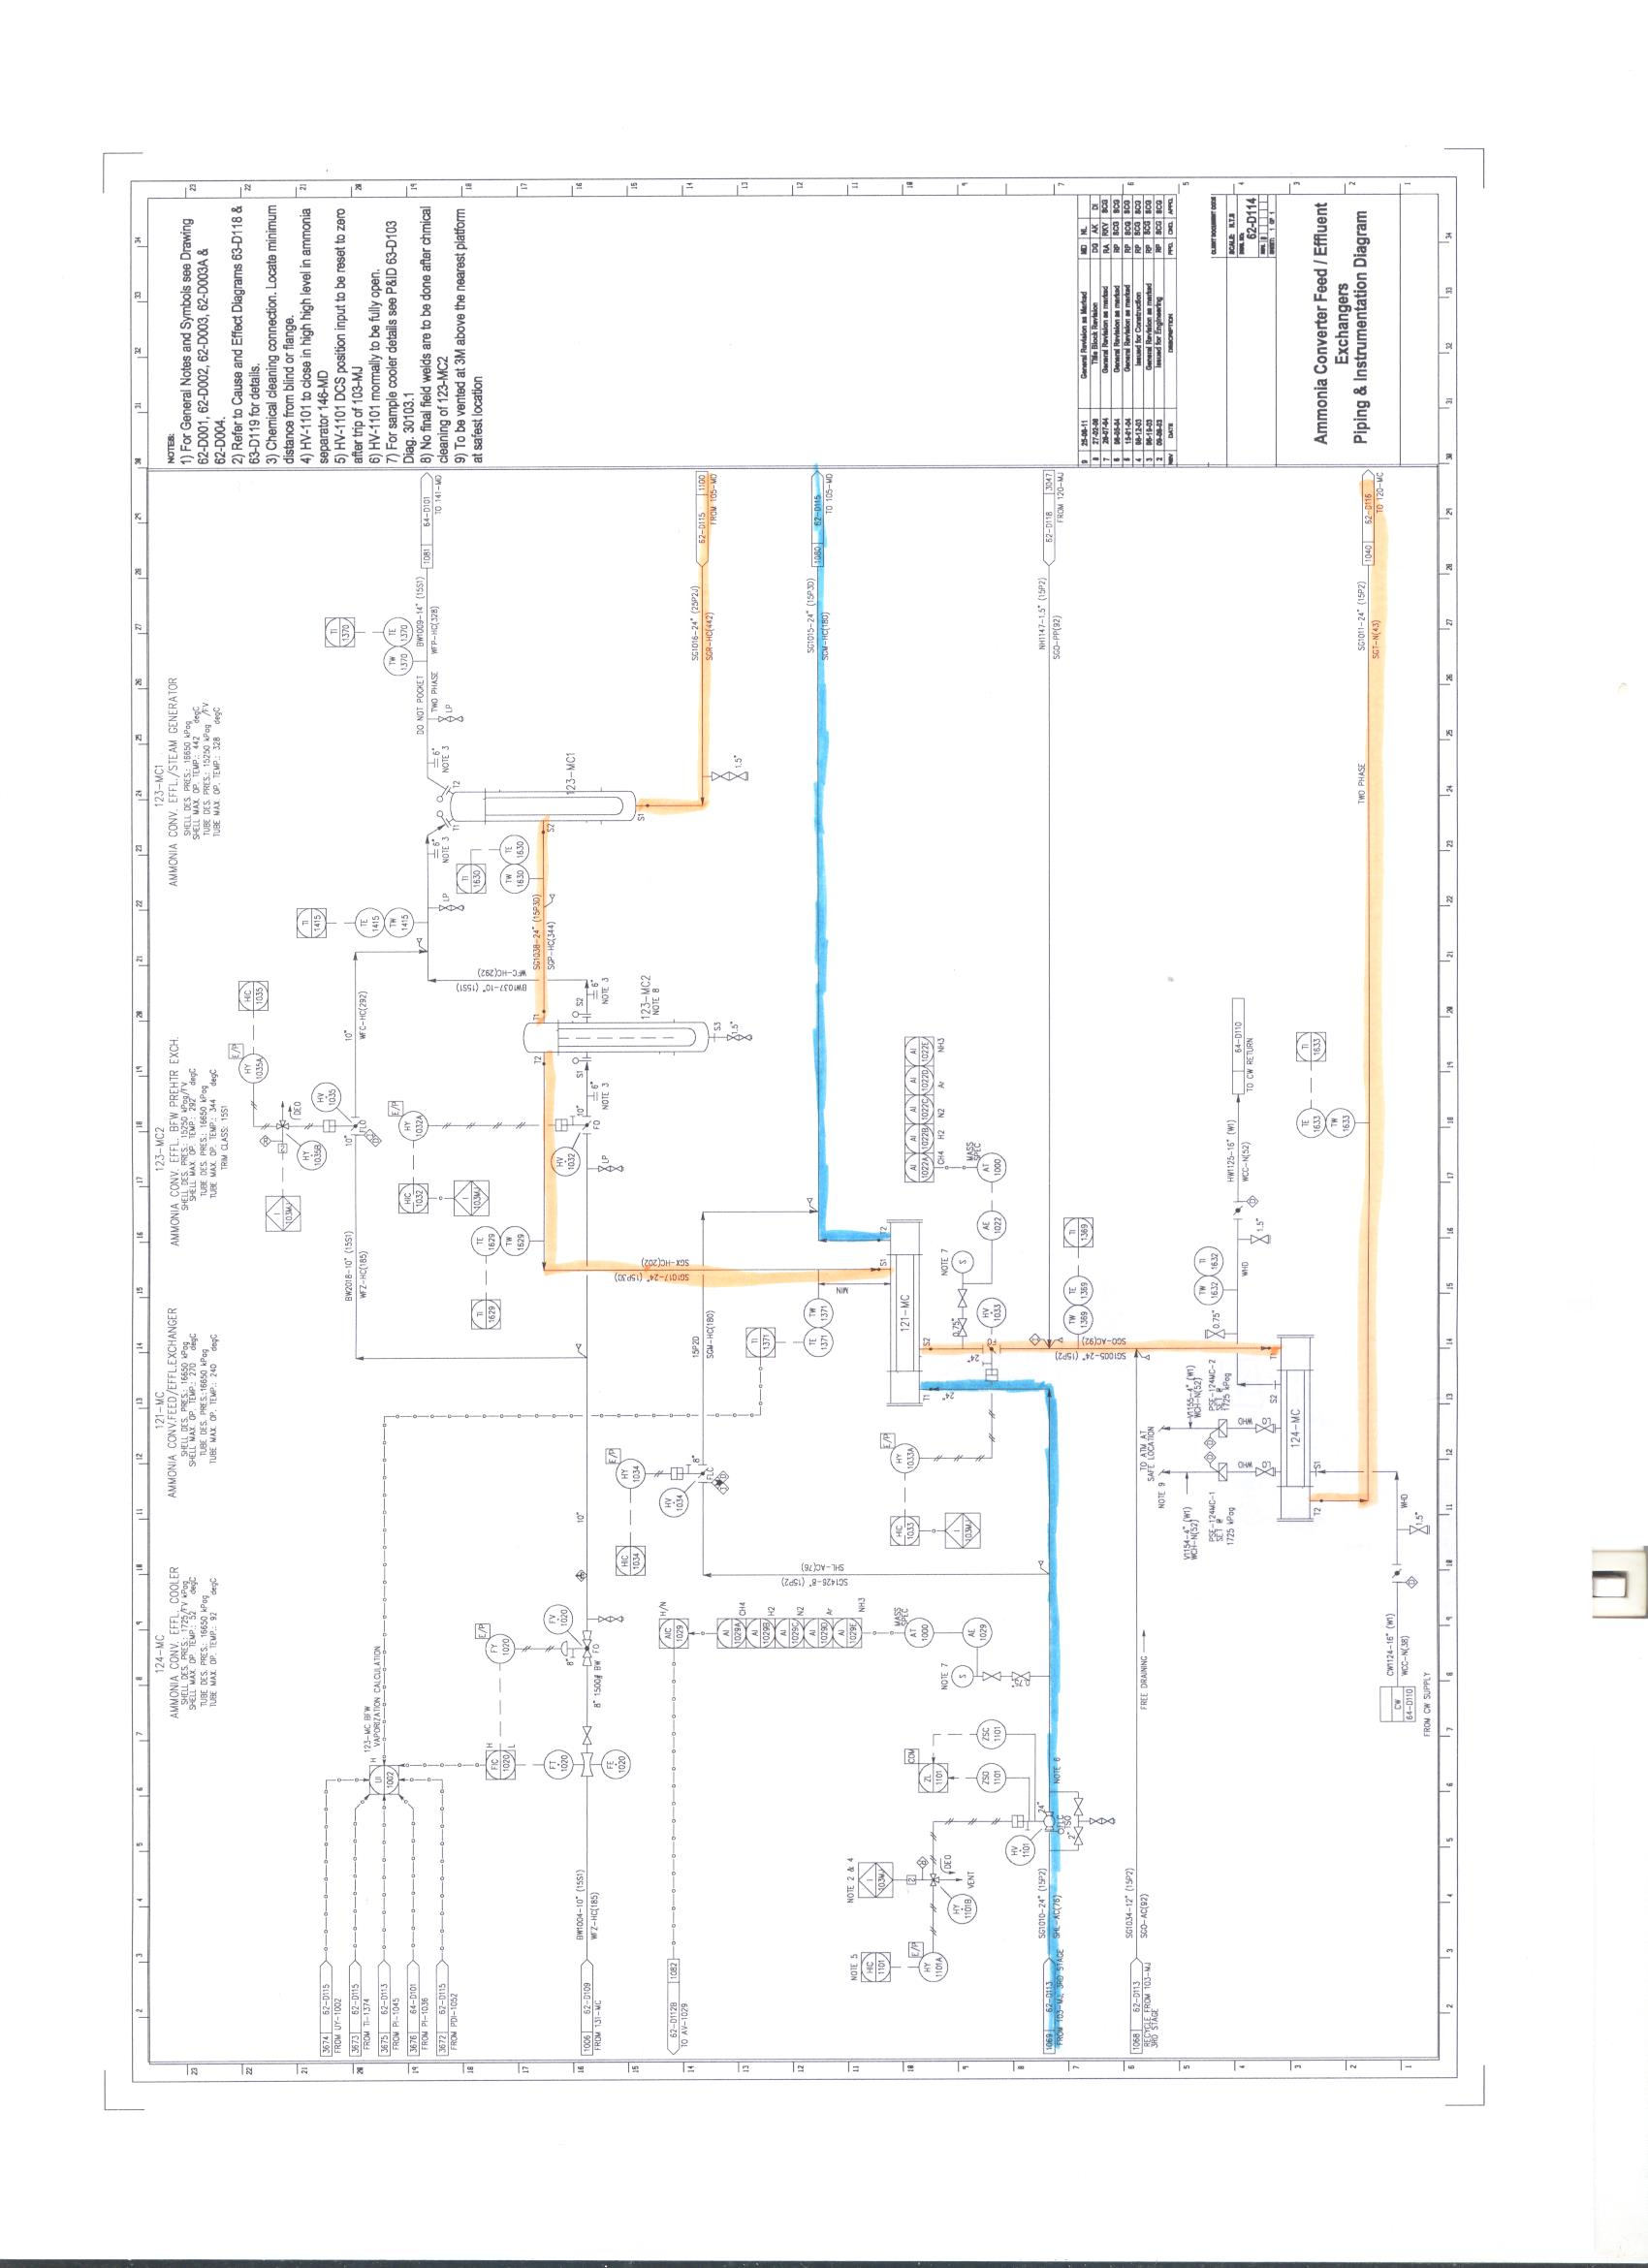
\includegraphics[scale=0.7]{img/scan2.jpg}

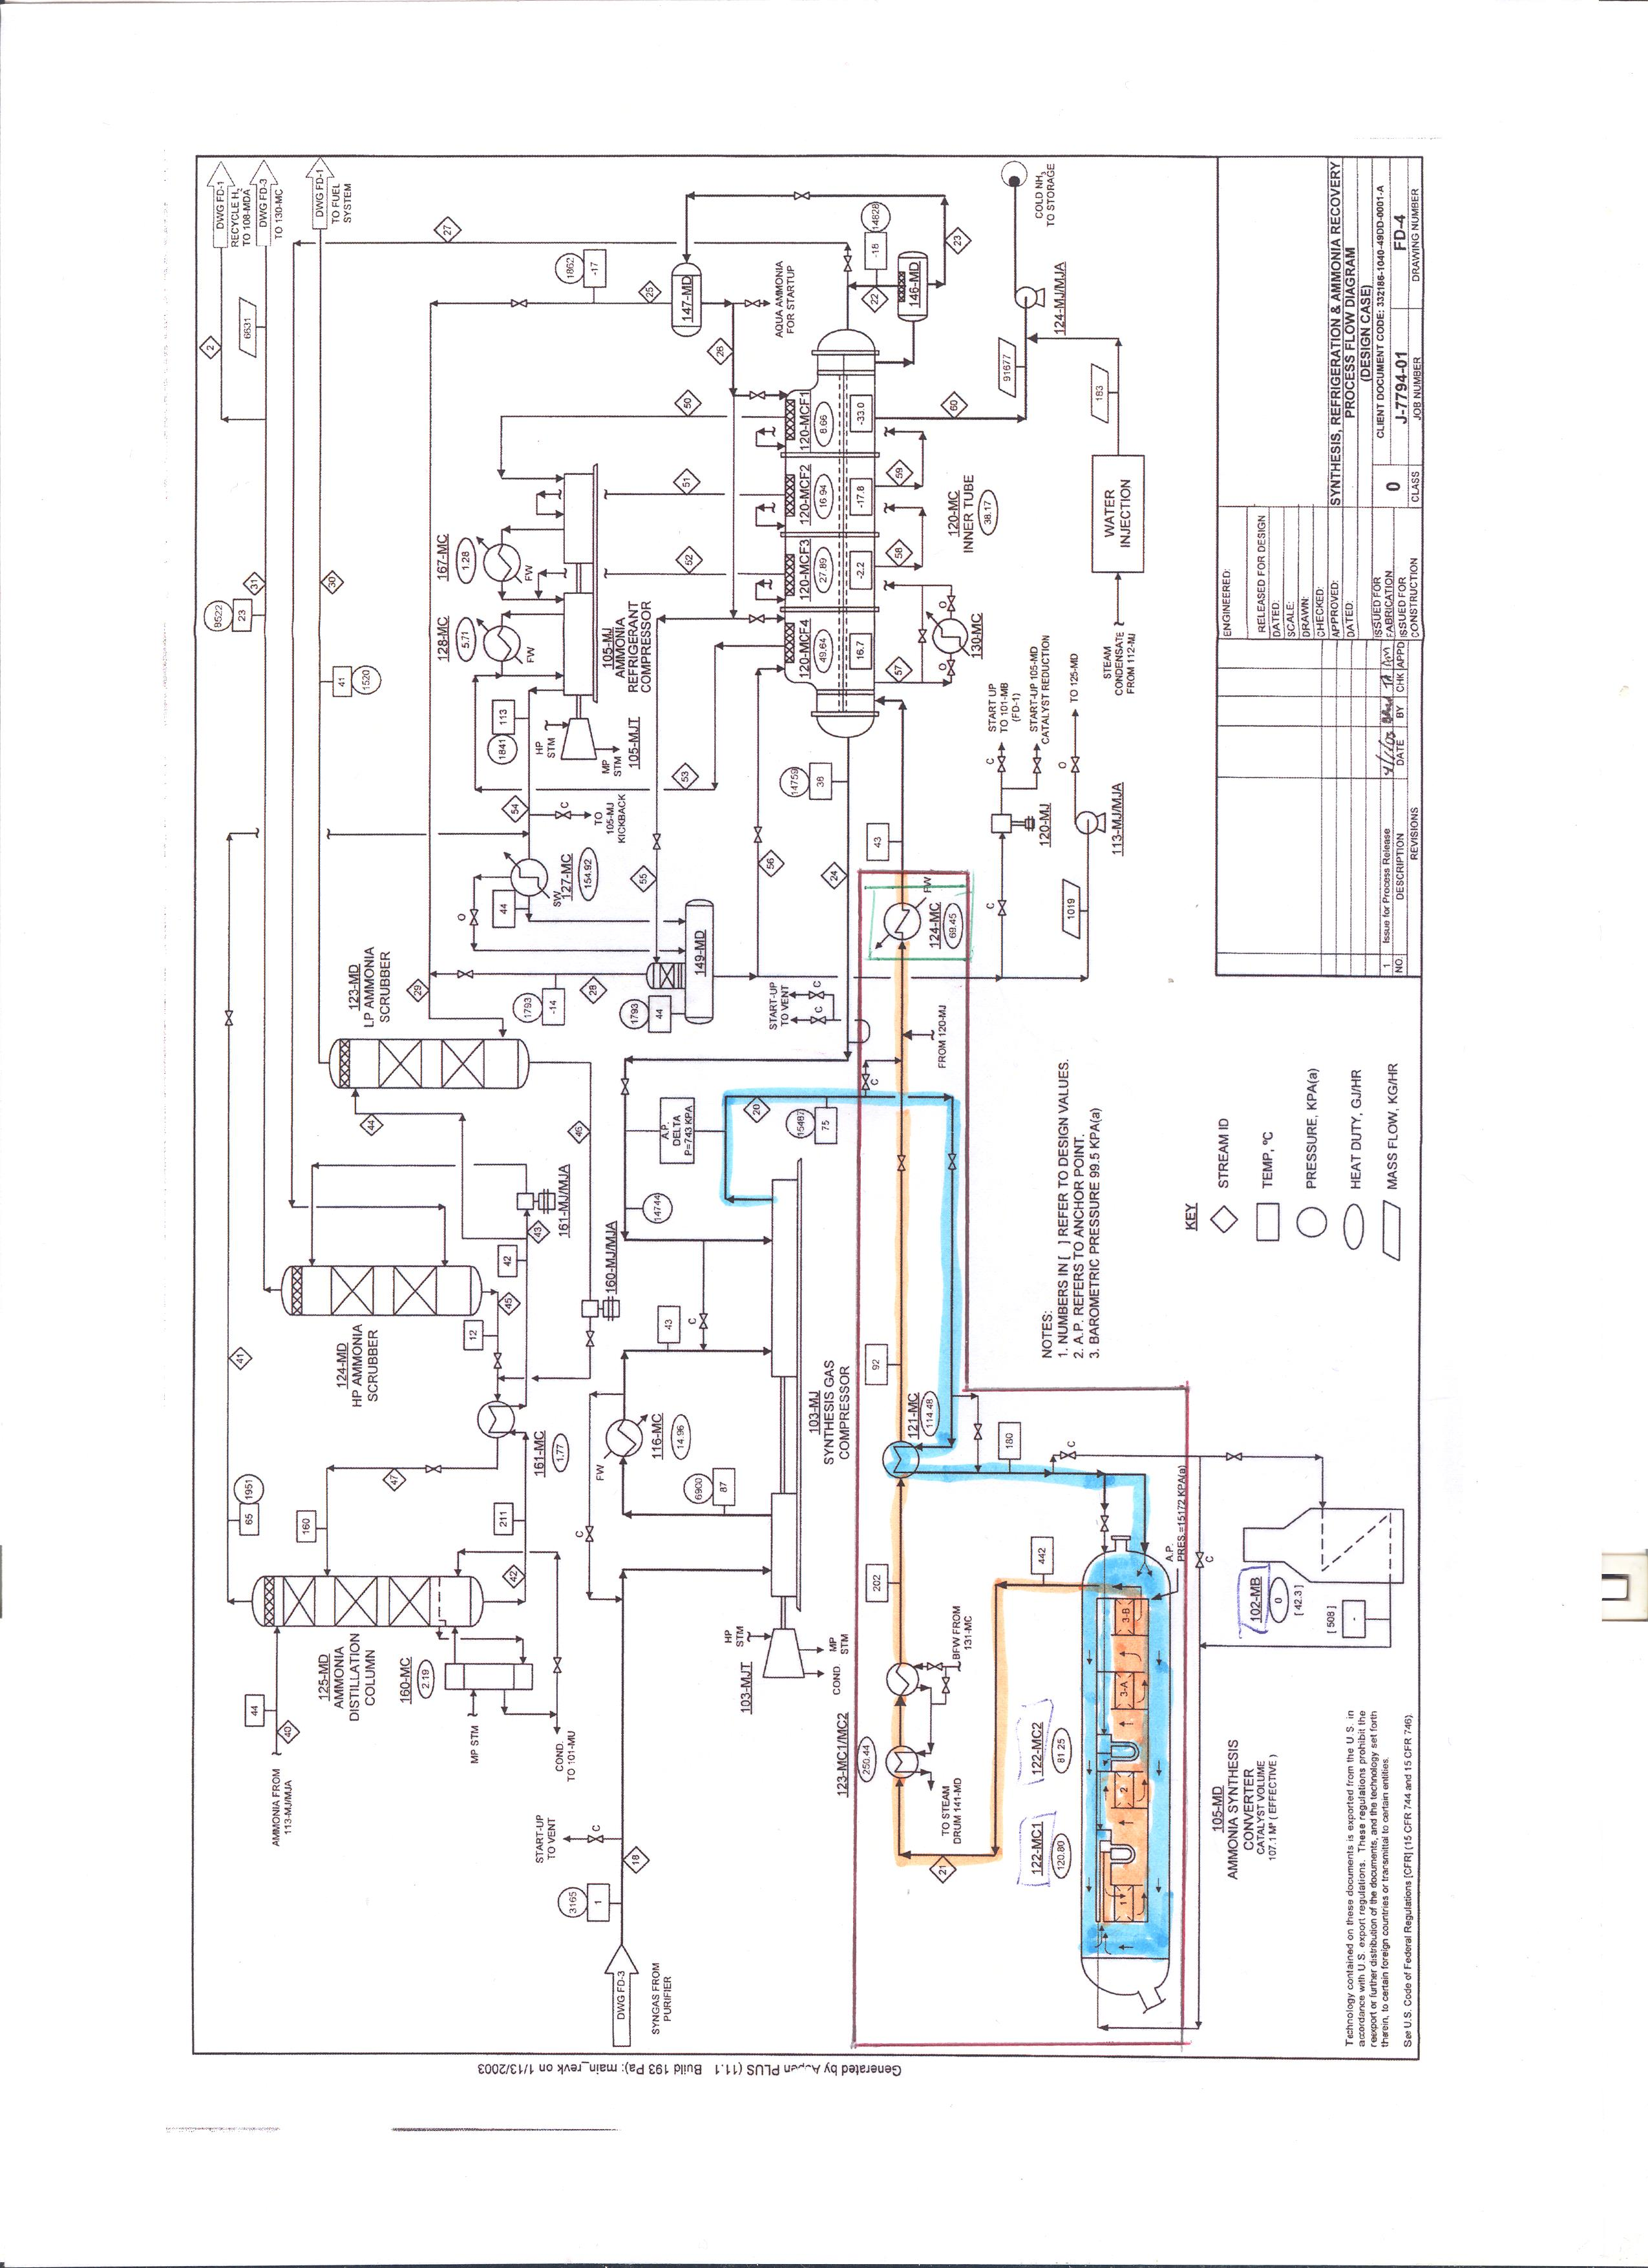
\includegraphics[scale=0.7]{img/scan3.jpg}
\end{center}

\end{document}
